\documentclass[a4paper]{article}
\usepackage[utf8]{inputenc}
\usepackage{amsmath}
\usepackage{amsfonts}
\usepackage{amssymb}
\setlength{\parindent}{0in}
\usepackage{fancyhdr}
\usepackage[sfdefault]{roboto}
\usepackage{roboto-mono}
\usepackage{listings,xcolor}
\usepackage{graphicx}

\definecolor{delim}{RGB}{20,105,176}
\definecolor{numb}{RGB}{106, 109, 32}
\definecolor{string}{rgb}{0.64,0.08,0.08}

\lstdefinelanguage{json}{
    numbers=left,
    numberstyle=\small,
    frame=single,
    rulecolor=\color{black},
    showspaces=false,
    showtabs=false,
    breaklines=true,
    postbreak=\raisebox{0ex}[0ex][0ex]{\ensuremath{\color{gray}\hookrightarrow\space}},
    breakatwhitespace=true,
    basicstyle=\ttfamily\small,
    upquote=true,
    morestring=[b]",
    stringstyle=\color{string},
    literate=
     *{0}{{{\color{numb}0}}}{1}
      {1}{{{\color{numb}1}}}{1}
      {2}{{{\color{numb}2}}}{1}
      {3}{{{\color{numb}3}}}{1}
      {4}{{{\color{numb}4}}}{1}
      {5}{{{\color{numb}5}}}{1}
      {6}{{{\color{numb}6}}}{1}
      {7}{{{\color{numb}7}}}{1}
      {8}{{{\color{numb}8}}}{1}
      {9}{{{\color{numb}9}}}{1}
      {\{}{{{\color{delim}{\{}}}}{1}
      {\}}{{{\color{delim}{\}}}}}{1}
      {[}{{{\color{delim}{[}}}}{1}
      {]}{{{\color{delim}{]}}}}{1},
}

\begin{document}
\begin{titlepage}
\begin{center}
\vspace*{1cm}

{\huge Requester}

\vspace{0.5cm}
Nástroj pro testování REST API

\vspace{1.5cm}

\textbf{David Nápravník}

\vfill

Zápočtová práce pro předměty\\
Jazyk C\# a platforma .NET - NPRG035 a\\
Pokročilé programování pro .NET I - NPRG038,\\
Programování uživatelských rozhraní v .NET - NPRG064


\vspace{0.8cm}


KDSS (Katedra distribuovaných a spolehlivých systémů)\\
Matematicko-fyzikální fakulta\\
Univerzita Karlova\\
26.07.2020

\end{center}
\end{titlepage}

\tableofcontents
\pagebreak

\section{Dokumentace požadavků}
    \subsection{Předpokládané využití}
        Program by měl primárně pomoci při vývoji REST API a
        jeho testování, pomocí posílání zkušebních dotazů (tkz. Requestů).\\
        Dále by měl pomoci se stahováním dat z webu, ať už manuálně, nebo 
        jako součást jiného programu, kdy lze mít předdefinovanovaou šablonu
        (tkz. Template) a tu obměňovat přes parametry, pro každý request.
    \subsection{Předpokládaná funkcionalita}
        Program musí umět posílat requesty typu \textbf{GET} a \textbf{POST}.\\
        V requestu se musí nechat měnit hlavička (tkz. Header), tělo a parametry
        v URL.
\section{Dokumentace architektury/designu}
    \subsection{Core}
        Jádrem je třída \textit{Requester} a další pomocné struktury.\\
        Nejdůležitější metodou jádra je \textit{Send}, která dostane
        co a kam odeslat a vrací odpověď ve formátu \textit{RequestResponse}
        obsahujcící status code, jak číselně tak jeho slovní formát,
        hlavičku, tělo odpovědi (tkz. Content) a čas od odeslání dotazu k jeho plnému přijetí.\\
    \subsection{GUI}
        Uživatelé se budou nejčastěji potýkat s GUI postaveným nad jádrem.\\
        GUI pro odeslání requestu schromáždí data od uživatele a předá je jádru,
        přesněji metodě Send, po příchodu odpovědi ji zpracuje a na contentu spustí
        automat (buď XML, nebo JSON), který ji LAZY zpracovává a vrací
        jak symbol zpracovat (text, řídící znak atd.), což je podstatné pro
        zobrazení "pretty" odpovéďi, která je obarvená a je indentovaná podle
        hloubky zanoření.
        \subsubsection{DataGrid}
            Seznam hodnot v hlavičce a parametrů pro url jsou zobrazeny pomoci
            DataGridu, což je vpodstatě tabulka do které uživatel může přidávat / 
            odebírat řádky, měnit jejich hodnoty a nebo je před odeláním zakázat.
        \subsubsection{Prohlížeč}
            Content lze zobrazit i tak jak by jej viděl prohlížeč.
            K tomu je použit defaultní prohlížeč z knihovny WPF,
            s podobným jádrem jako prohlížeč IE9.
        \subsubsection{Design}
            Uživatelské rozhraní se nese v duchu Material designu vytvořeného
            společností Google. Dbá na jednoduché, přehledné a uživatelsky přívětivé
            prostředí. Všechny části jsou responzivní a připravené na různé velikosti displaye.
            Barvy v GUI jsou v tmavém režimu, jež šetří oči při dlouhodobějším používaní. 
    \subsection{CLI}
        CLI verze programu je Headless a tudíž nepožaduje po svém spuštění, žádnou interakci
        a sama vždy skončí, buď neúspěšně, nebo vrátí do konzole odpověď.
        Popř. uloží tělo requestu do souboru.\\
        Lze spustit buď s Templatem nebo s parametry, nebo s obojím zároveň,
        s tím že nejdříve se načte konfirurace z Templeatu a pak je doplněna /
        pozměněna daty z parametrů. 
\section{Technická dokumentace}
    \subsection{HTTP Client}
        Pro komunikaci samotnou byla použita knihovna \textit{System.Net.Http}.\\
        Requesty jsou typu SEND a POST a posílají se asynchronně.
    \subsection{Algoritmy}
        \subsubsection{Automat na parsování JSON}
            Automat přijímá pokaždé jeden znak a vrací jakého typu znak je
            a hloubku zanoření.\\
            Typy znaku:
            \begin{itemize}
                \item objectBracket
                \item arrayBracket
                \item paramName
                \item JSONstring
                \item number
                \item logic
                \item specialChar
                \item whitespace
            \end{itemize}
        \subsubsection{Automat na parsování XML}
            Automat přijímá jeden znak a vrací v jakém stavu automat je a hloubku zanoření
            (odhad hloubky v případě nedeterministického stavu).\\
            narozdíl od Automatu pro JSON, je tento automat nedeterministický 
            a to v případě znaku "<" protože nemůžeme vědět, zda je to začátek
            nového tagu, nebo ukončení starého, z čehož nelze vyvodit hloubka zanoření a 
            je třeba počkat na další symbol.\\
            Stavy automatu:
            \begin{itemize}
                \item left
                \item tagName
                \item whitespace
                \item metadata
                \item right
                \item data
                \item slash
            \end{itemize}			
    \subsection{Ukládání Templateu}
        Templaty se ukládají ve formátu JSON a obsahují vše co uživatel zadá do rozhraní GUI.\\
        Ukázka templeatu requestu pro získání IP odesílatele:
        \begin{lstlisting}[language=json,numbers=none,frame=none]
{
    "url": "https://api.ipify.org",
    "method": "GET",
    "parameters": [
    ],
    "header": [
        {
        "active": true,
        "key": "Content-Type",
        "value": "application/json"
        }
    ],
    "content": ""
}            
            \end{lstlisting}
    \subsection{Testy}
        Všechny public metody z Jádra mají vlastní testy, jež ověřují 
        korektnost výstupu jak pro běžné použití, tak i pro pár edge-*case případů.
\section{Uživatelská dokumentace}
    \subsection{Rozhraní GUI}
        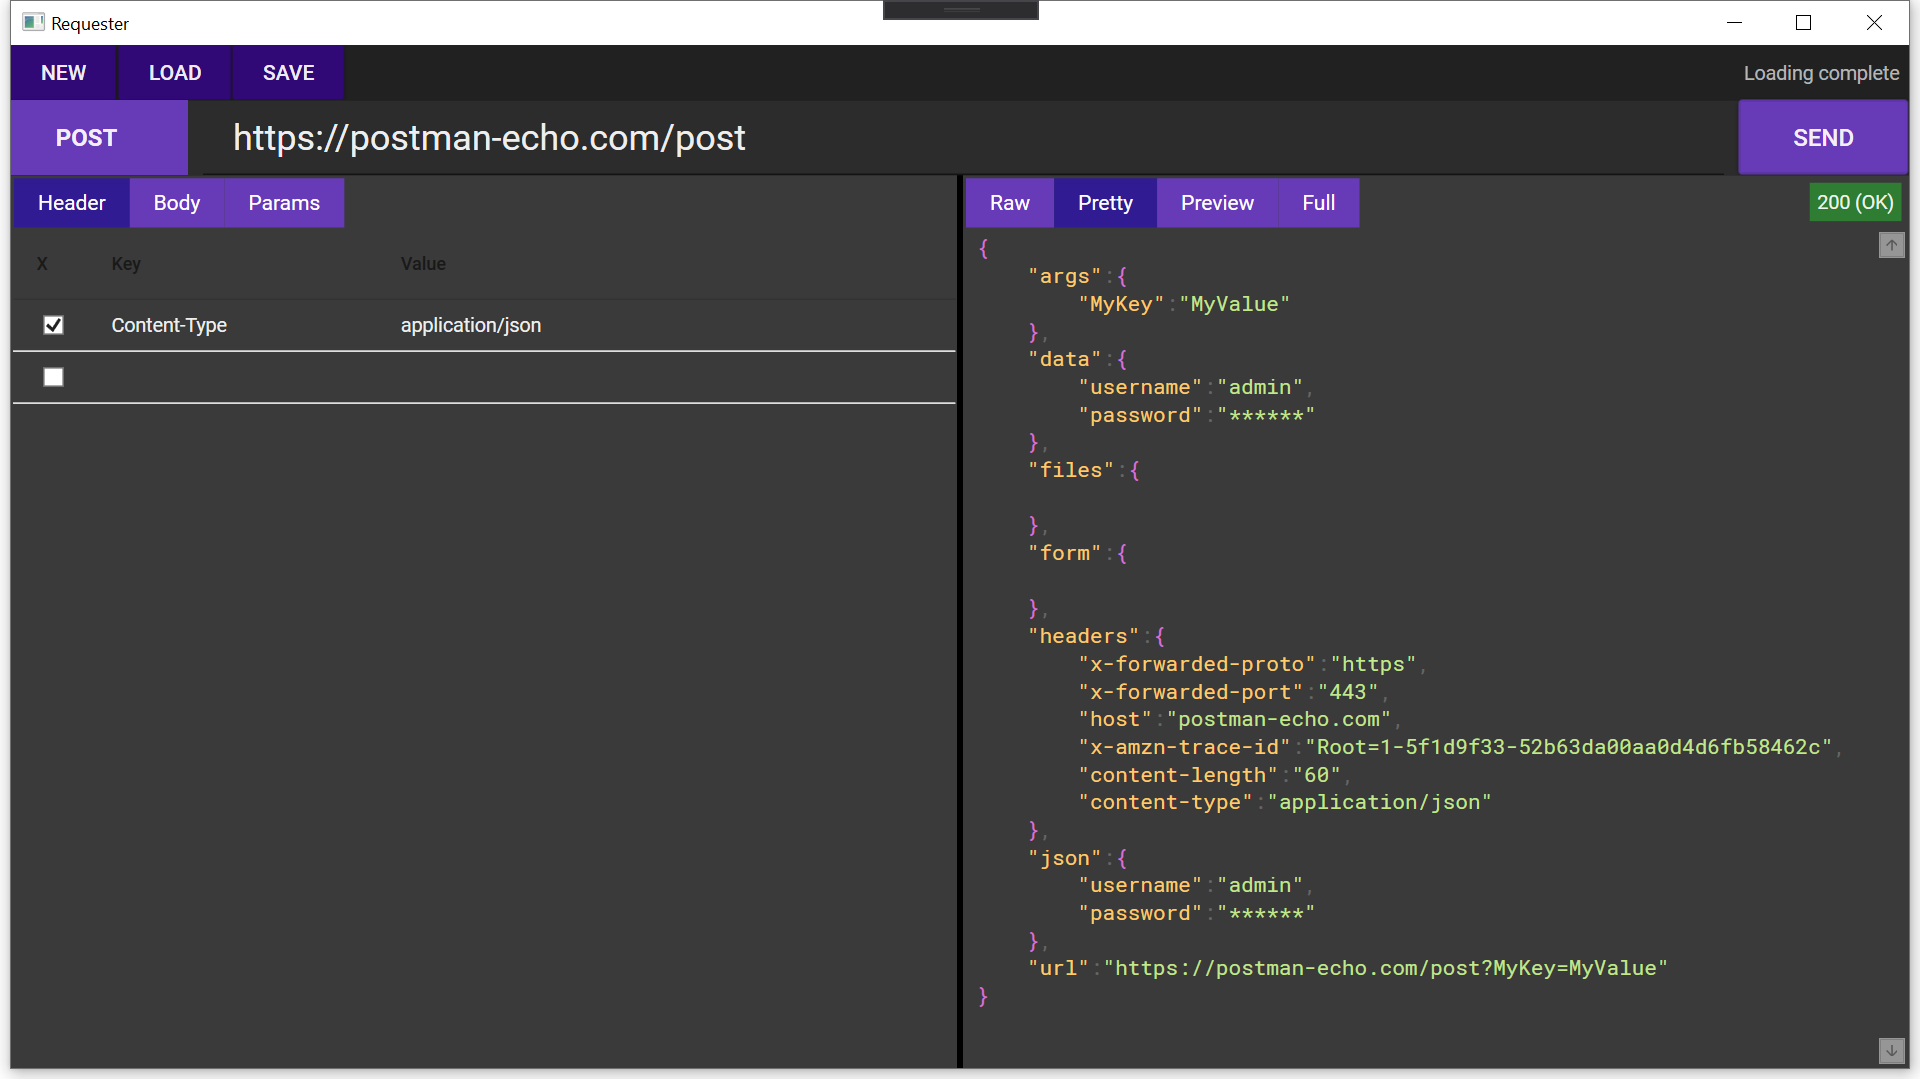
\includegraphics[width=\textwidth]{mainPage.PNG}
        V horní části vidíme 3 tlačítka pro ukládání a načítání templeatu a
        pole s informacemi pro uživatele v pravém rohu\\
        Níže je výběrové pole pro typ requestu (POST nebo GET).
        Uprostřed je místo pro URL. Program přijímá i url bez udání protokolu.\\
        Tlačítko SEND pak odesílá request.\\
        Levá spodní část je vstupní a pravá výstupní.\\
        \\
        Vlevo vidíme tabulku, kde každý řádek je jedna položka v hlaviččce.
        Řádky mažeme pomocí označení a klávesy Del. Nové řádky se
        přidávají automaticky.\\
        \\
        Vpravo vidíme výsledek requestu, tak jak jej automat sparsoval a
        kód přijatého requestu. (200 OK)\\
        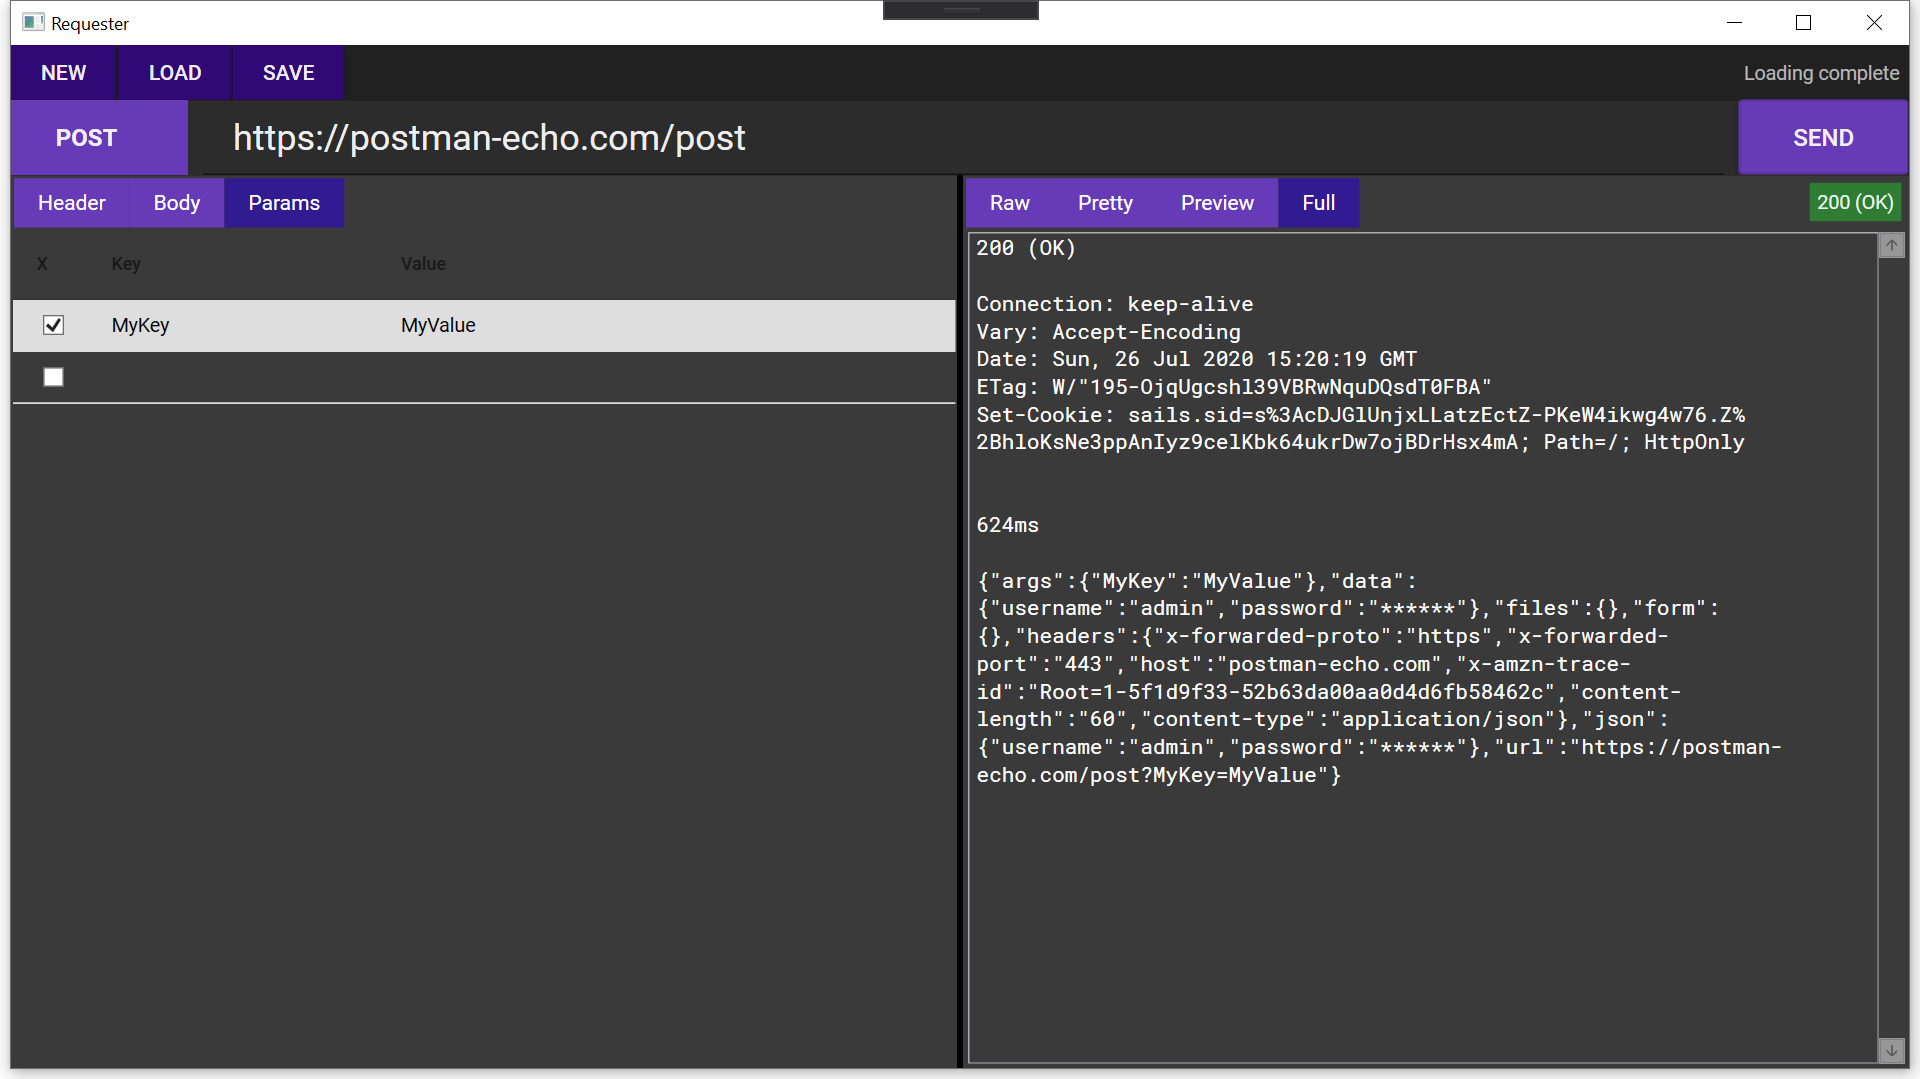
\includegraphics[width=\textwidth]{thirdPage.PNG}
        Vlevo vidíme podobnout tabulku jako pro zadávání hlavičky.\\
        Vpravo je zobrazen celý výsledek requestu \dots Stavový kód, 
        Hlavička, čas pro přijetí požadavku a tělo.\\
        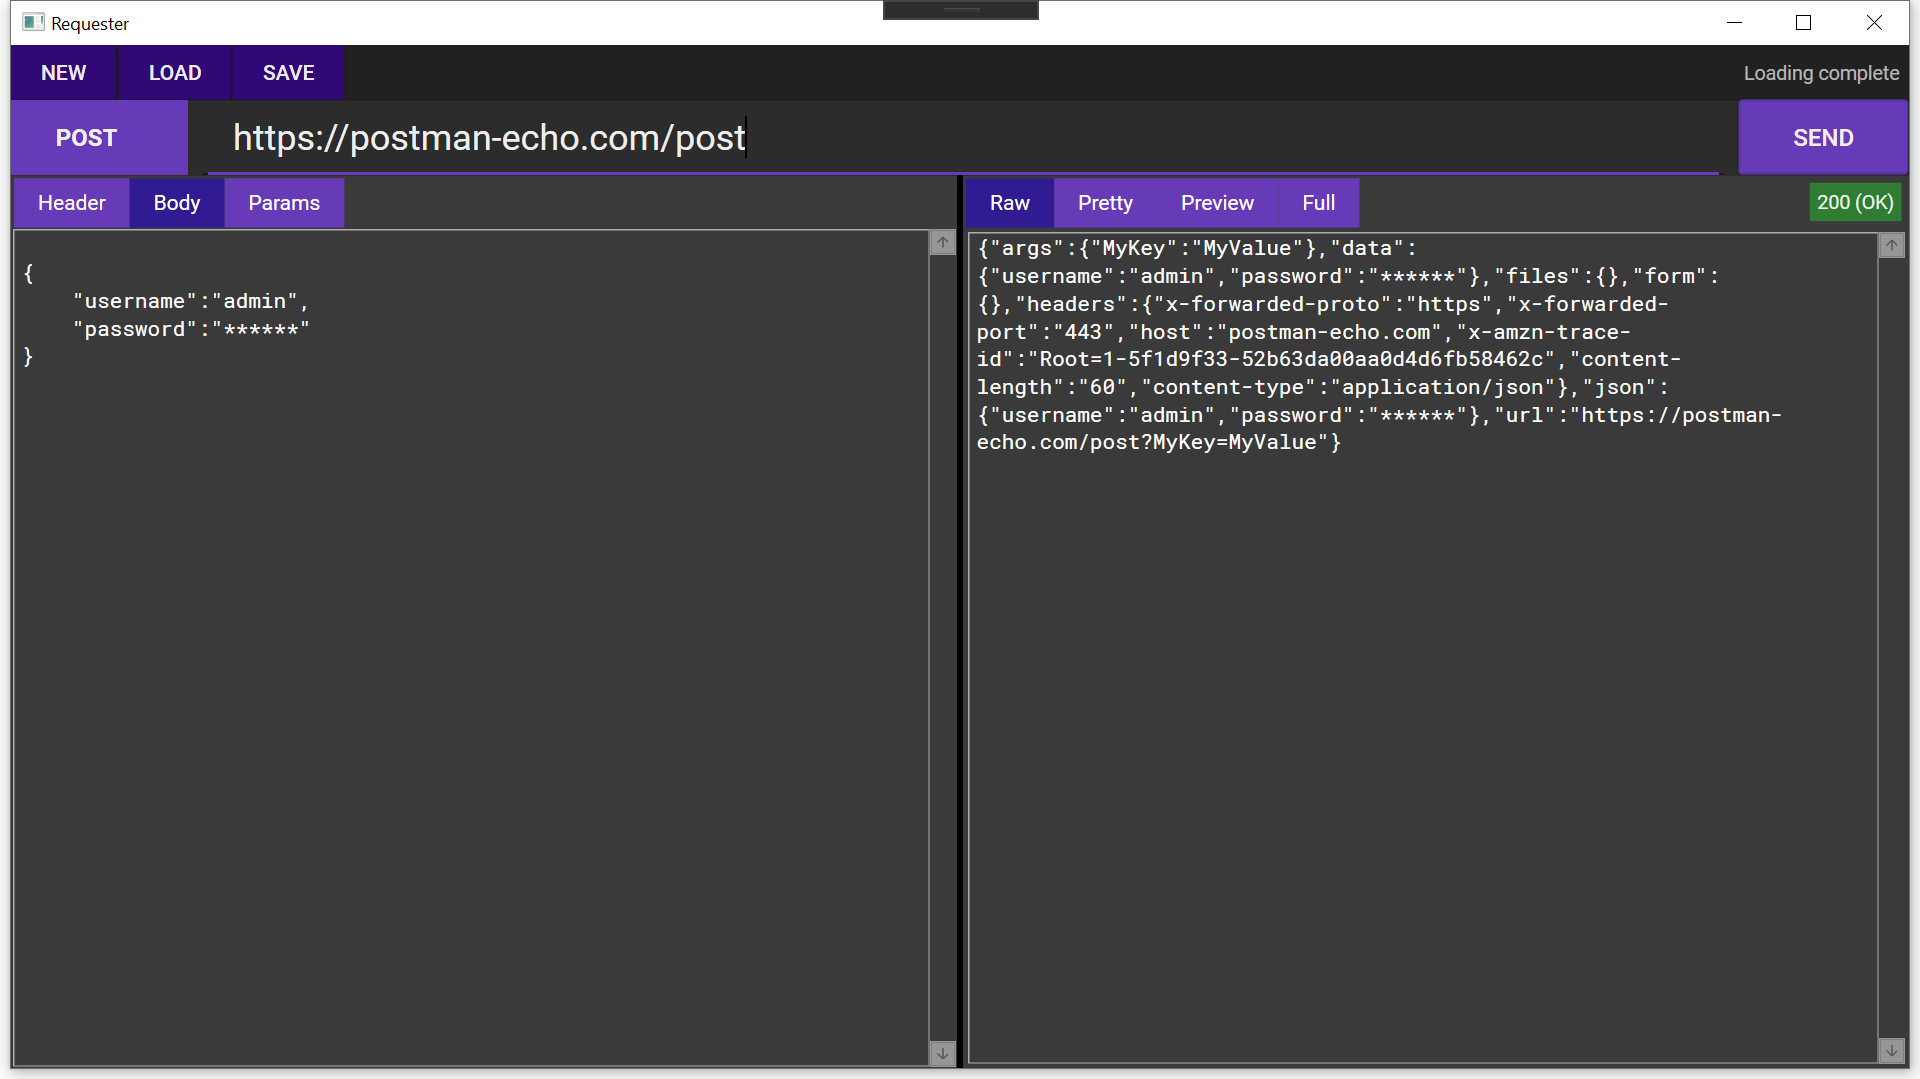
\includegraphics[width=\textwidth]{secondPage.PNG}
        Tělo requestu (tkz. Body) je čistě text a tak se i zpracovává.
        Pokud chtete odesílat JSON nebo XML, je třeba změnit datový typ v hlavičce.
        Přesněji položku "Content-Type" změnit například na "application/json".\\
        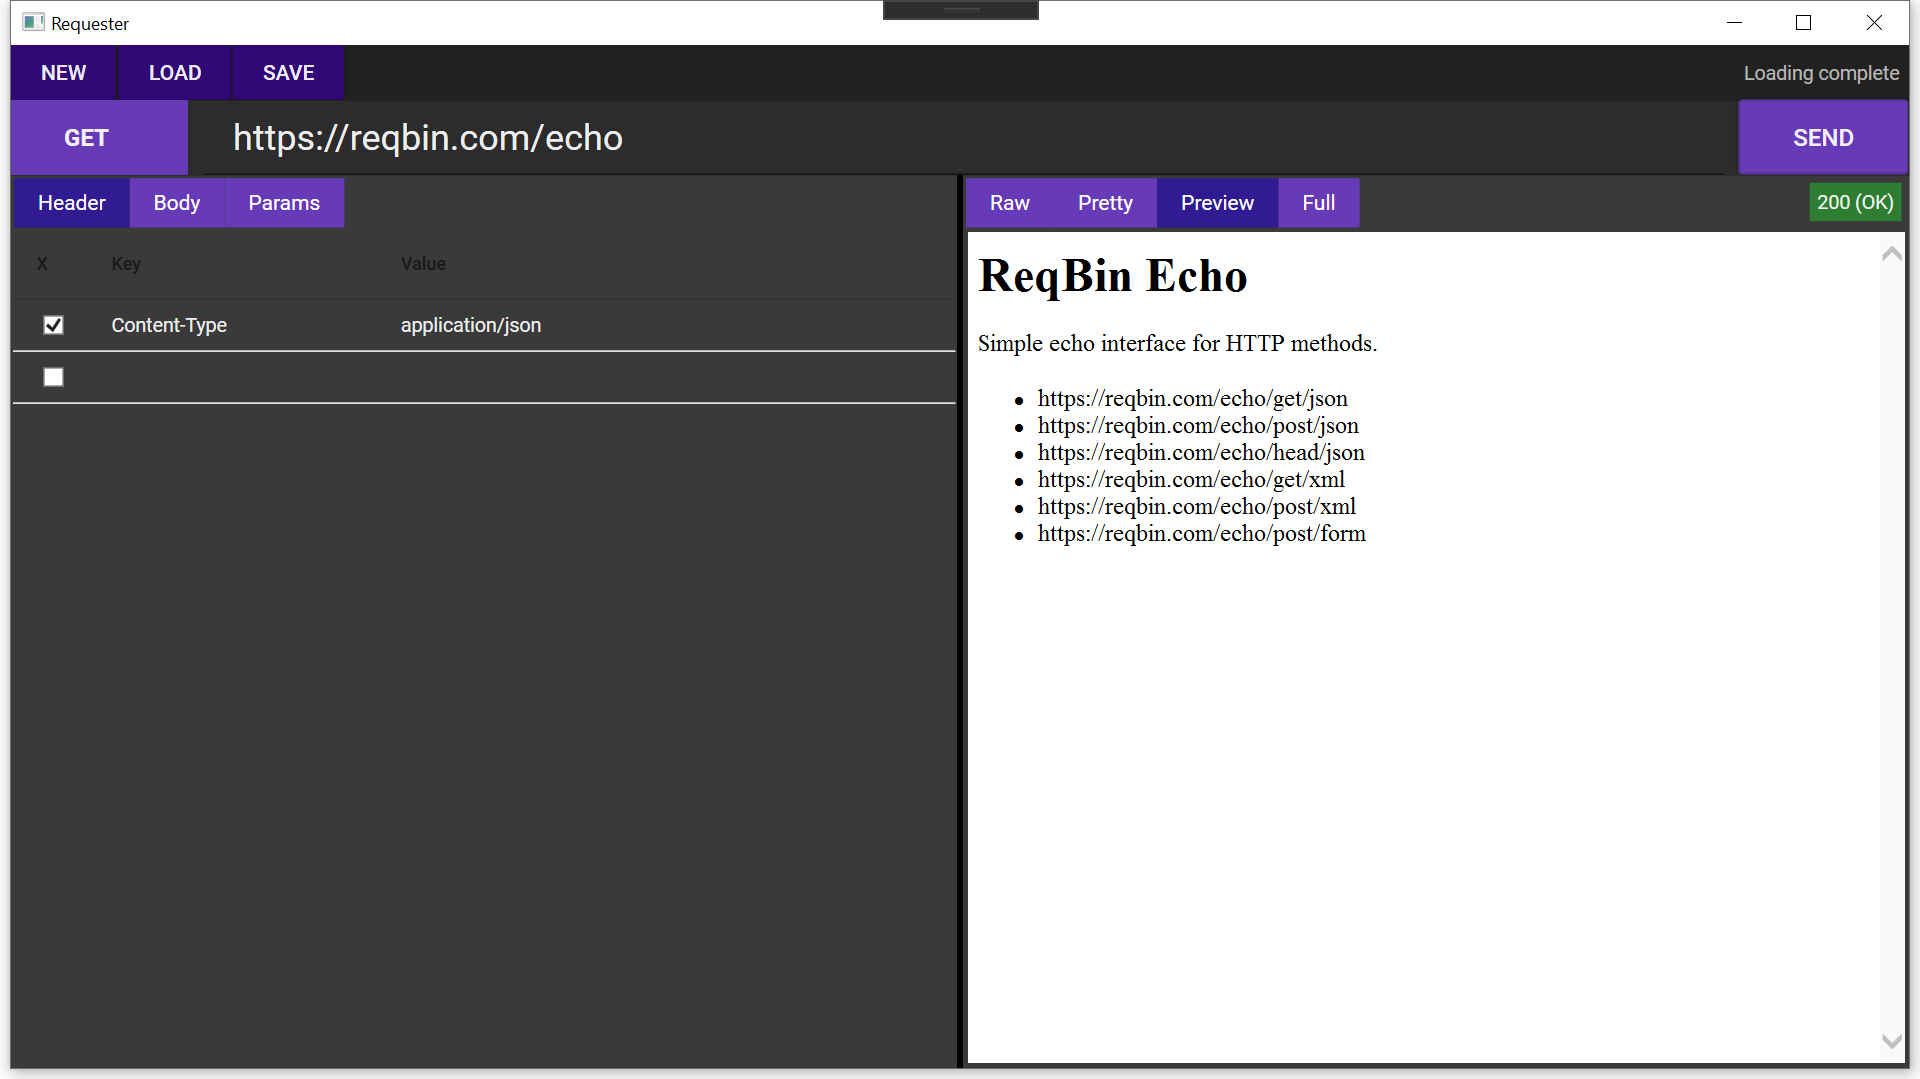
\includegraphics[width=\textwidth]{Preview.PNG}
        V případě potřeby je možné zobrazit odpověď i tak jak ji vidí
        uživatel v prohlížeči a to v záložce Preview.
        \subsubsection{Ukládání Templateu}
            Pro uložení Templatu stačí zmáčnout tlačítko SAVE a vybrat cílový adresář.\\
            Pro načtení slouží tlačitko LOAD, templaty se vždy ukládají s koncovkou JSON.
        \subsubsection{Klávesové zkratky}
            \begin{itemize}
                \item Ctrl + S $\rightarrow$ Uložení templeatu do souboru
                \item Ctrl + O $\rightarrow$ Načtení templeatu ze souboru
                \item Ctrl + Enter $\rightarrow$ Odeslání Requestu
            \end{itemize}
    \subsection{Rozhraní CLI}
    \textbf{Ukázka použití:}
        \begin{lstlisting}[language=bash]
> .\bin\Debug\Requester.exe -t '.\sample requests\GET IP.json'
200 (OK)

Connection: keep-alive
Vary: Origin
Date: Sun, 26 Jul 2020 15:48:41 GMT
Server: Cowboy
Via: 1.1 vegur

530ms

93.99.225.88
        \end{lstlisting}
        \textbf{Argumenty:}
        \begin{itemize}
            \item[] -o    output file 
            \item[] -t    template 
            \item[] -m    method 
            \item[] -u    url 
            \item[] -c    content 
            \item[] -h    header 
        \end{itemize}
        V případě uvedení argumentu -o se ukládá pouze tělo
        odpovědi, nikolov celý záznam (hlavička atd.).


\end{document}